\documentclass{tufte-handout}

%\geometry{showframe}% for debugging purposes -- displays the margins
\usepackage{lmodern}
\geometry{
	left=13mm, % left margin
	textwidth=130mm, % main text block
	marginparsep=8mm, % gutter between main text block and margin notes
	marginparwidth=55mm % width of margin notes
}
\usepackage{framed}
\usepackage{amsmath}
\usepackage{amssymb}
\usepackage{amsthm}

% Set up the images/graphics package
\usepackage{graphicx}
\setkeys{Gin}{width=\linewidth,totalheight=\textheight,keepaspectratio}
\graphicspath{{graphics/}}

\title{	
	\normalfont\normalsize 
	{PHIL 120 - Winter 2025} \\[0.75em]  % Your university, school and/or department name(s)
	\huge Course Notes% The assignment title
}\author{Alex Diep} % Your name
\date{\vspace{-5pt}\normalsize \today} % Today's date or a custom date

% The following package makes prettier tables.  We're all about the bling!
\usepackage{booktabs}

% The units package provides nice, non-stacked fractions and better spacing
% for units.
\usepackage{units}

% The fancyvrb package lets us customize the formatting of verbatim
% environments.  We use a slightly smaller font.
\usepackage{fancyvrb}
\fvset{fontsize=\normalsize}

% Small sections of multiple columns
\usepackage{multicol}

% Provides paragraphs of dummy text
\usepackage{lipsum}

% These commands are used to pretty-print LaTeX commands
\newcommand{\doccmd}[1]{\texttt{\textbackslash#1}}% command name -- adds backslash automatically
\newcommand{\docopt}[1]{\ensuremath{\langle}\textrm{\textit{#1}}\ensuremath{\rangle}}% optional command argument
\newcommand{\docarg}[1]{\textrm{\textit{#1}}}% (required) command argument
\newenvironment{docspec}{\begin{quote}\noindent}{\end{quote}}% command specification environment
\newcommand{\docenv}[1]{\textsf{#1}}% environment name
\newcommand{\docpkg}[1]{\texttt{#1}}% package name
\newcommand{\doccls}[1]{\texttt{#1}}% document class name
\newcommand{\docclsopt}[1]{\texttt{#1}}% document class option name

\usepackage{fancyhdr} % Custom headers and footers
\pagestyle{fancyplain} % Makes all pages in the document conform to the custom headers and footers
\fancyhead{} % No page header - if you want one, create it in the same way as the footers below
\fancyfoot[L]{} % Empty left footer
\fancyfoot[C]{} % Empty center footer
\fancyfoot[R]{\thepage} % Page numbering for right footer

% \usepackage{sectsty} % Allows customizing section commands
% \allsectionsfont{\normalfont \bfseries} % Make all sections centered, the default font and small caps
\usepackage{titlesec}
% Customize section titles
\titleformat{\section}
  {\normalfont\LARGE\bfseries} % Format for \section: large font, bold
  {\thesection}{1em}{}

\titleformat{\subsection}
  {\normalfont\large\bfseries} % Format for \subsection: large font, bold
  {\thesubsection}{1em}{}

\let\biconditional\leftrightarrow

%--------Theorem Environments--------
% \theoremstyle{plain} --- default
% Custom theorem styles
\newtheoremstyle{definition}
  {\topsep}   % ABOVESPACE
  {\topsep}   % BELOWSPACE
  {\itshape}  % BODYFONT
  {0pt}       % INDENT (empty value is the same as 0pt)
  {\bfseries} % HEADFONT
  {.}         % HEADPUNCT
  {5pt plus 1pt minus 1pt} % HEADSPACE
  {}          % CUSTOM-HEAD-SPEC

\newtheoremstyle{example}
  {\topsep}   % ABOVESPACE
  {\topsep}   % BELOWSPACE
  {}  % BODYFONT
  {0pt}       % INDENT (empty value is the same as 0pt)
  {\itshape} % HEADFONT
  {.}         % HEADPUNCT
  {5pt plus 1pt minus 1pt} % HEADSPACE
  {\thmname{#1}\thmnumber{\textit{ #2}}\thmnote{ (#3)}}          % CUSTOM-HEAD-SPEC


\newtheorem{thm}{Theorem}
\newtheorem{cor}[thm]{Corollary}
\newtheorem{prop}[thm]{Proposition}
\newtheorem{facts}[thm]{Facts}
\newtheorem{fact}[thm]{Fact}
\newtheorem{clm}[thm]{Claim}
\newtheorem{lem}[thm]{Lemma}
\newtheorem{conj}[thm]{Conjecture}
\newtheorem{quest}[thm]{Question}

% \theoremstyle{definition}
% \newtheorem{defn}[thm]{Definition}
% \newtheorem{defns}[thm]{Definitions}
% \newtheorem{con}[thm]{Construction}
% \newtheorem{exmp}[thm]{Example}
% \newtheorem{thms}[thm]{Examples}
% \newtheorem{notn}[thm]{Notation}
% \newtheorem{notns}[thm]{Notations}
% \newtheorem{addm}[thm]{Addendum}
% \newtheorem{exer}[thm]{Exercise}

% \theoremstyle{remark}
% \newtheorem{rem}[thm]{Remark}
% \newtheorem{rems}[thm]{Remarks}
% \newtheorem{warn}[thm]{Warning}
% \newtheorem{sch}[thm]{Scholium}

\theoremstyle{definition}
\newtheorem{defn}{Definition}
\newtheorem{defns}{Definitions}
\newtheorem{con}{Construction}

\theoremstyle{example}
\newtheorem{exmp}{Example}
\newtheorem{exmps}{Examples}
\newtheorem{notn}{Notation}
\newtheorem{notns}{Notations}
\newtheorem{addm}{Addendum}
\newtheorem{exer}{Exercise}

\theoremstyle{remark}
\newtheorem{rem}{Remark}
\newtheorem{rems}{Remarks}
\newtheorem{warn}{Warning}
\newtheorem{sch}{Scholium}

\usepackage{tocloft} % Add this line to include the tocloft package
\renewcommand{\cftsecfont}{\normalfont \bfseries} % Section titles in normal font
\renewcommand{\cftsubsecfont}{\normalfont} % Subsection titles in normal font
\renewcommand{\cftsecleader}{\cftdotfill{\cftdotsep}} % Section leaders
\renewcommand{\cftsubsecleader}{\cftdotfill{\cftdotsep}} % Subsection leaders
\renewcommand{\cftsubsecpagefont}{\bfseries} % Subsection page numbers in bold


\usepackage{enumitem} % Add this line in the preamble if not already included

\begin{document}

\maketitle% this prints the handout title, author, and date

\begin{abstract}
  These are distilled notes taken from \textit{forallx CALGARY An Introduction to Formal Logic} taught by Paolo Verdini.
\end{abstract}

\tableofcontents
\newpage

\pagebreak
\section{Key Notions of Logic}
\subsection{Arguments}
\begin{defn}
  A \textbf{sentence} is a statement that can be true or false.
\end{defn}
\begin{exmp}
  The following are sentences:
  \begin{enumerate}[leftmargin=3\parindent]
    \item The cat is on the mat.
    \item Rhubarb is tasty.
  \end{enumerate}
  The following are not sentences:
  \begin{enumerate}[leftmargin=3\parindent]
    \item Are you sleepy yet?
    \item Go to your room!
    \item Ouch!
  \end{enumerate}
\end{exmp}
\begin{defn}
  An \textbf{argument} is a sequence of statements. One of these statements is the \textbf{conclusion} and the remaining statements are the \textbf{premises}.
\end{defn}
\begin{exmp}
  Consider the following argument:
  \begin{align*}
     & \textbf{Premise 1: } \text{Either the butler or the cook did it.} \\
     & \textbf{Premise 2: } \text{The butler did not do it.}             \\
     & \textbf{Conclusion: } \therefore \text{The cook did it.}
  \end{align*}
\end{exmp}
\begin{defn}
  A \textbf{premise indicator word} is a word that indicates that what follows is a premise of an argument. Some common premise indicator words include \textit{since}, \textit{because}, \textit{given that}, \textit{as}, \textit{for}, \textit{seeing that}, \textit{in as much as}
\end{defn}
\begin{defn}
  A \textbf{conclusion indicator word} is a word that indicates that what follows is the conclusion of an argument. Some common conclusion indicator words include \textit{therefore}, \textit{thus}, \textit{so}, \textit{hence}, \textit{consequently}, \textit{accordingnly}
\end{defn}

\subsection{The Scope of Logic}
\begin{framed}
  \begin{defn}
    A sentence $\mathcal{A}$ is a \textbf{consequence} of the set of sentences $\mathcal{B} = \{B_1, B_2, \ldots, B_n\}$ if and only if it is impossible for all of the sentences in $\mathcal{B}$ to be true while $\mathcal{A}$ is false.
  \end{defn}
\end{framed}
\begin{framed}
  \begin{defn}
    An argument is \textbf{valid} or \textbf{deductively valid} if and only if the conclusion is a consequence of the premises. \\ An argument is \textbf{invalid} if and only if the conclusion is not a consequence of the premises.
  \end{defn}
\end{framed}
\begin{exmp}
  Can a valid argument be made invalid by the addition of a new premise? \\[1em]
  No. If an argument is valid, then by definition, it's impossible for the premises to be true and the conclusion false. This implies there is at least one presmise that is false when the conclusion is false. Thus, adding a new premise will not change the fact that not all premises can be true while the conclusion is false.
\end{exmp}
\begin{defn}
  A \textbf{counterexample} is an example that shows that an argument is invalid.
\end{defn}
\begin{defn}
  An argument is \textbf{nomologically valid} if the conclusion is a consequence of the premises in virtue of the laws of nature.
\end{defn}
\begin{exmp}
  Consider the following argument:
  \begin{align*}
     & \textbf{Premise 1: } \text{The spaceship took six hours to reach Jupiter from Tycho space station}                        \\
     & \textbf{Conclusion: } \therefore \text{The distance between Jupiter and Tycho space station is} \leq \text{6 light hours}
  \end{align*}
  This argument is nomologically valid.
\end{exmp}
\begin{defn}
  An argument is \textbf{conceptually valid} if there are no counterexamples that don't violate conceuptual connections between the premises words.
\end{defn}
\begin{exmp}
  Consider the following argument:
  \begin{align*}
     & \textbf{Premise 1: } \text{Priya is an opthalmologist}         \\
     & \textbf{Conclusion: } \therefore \text{Priya is an eye doctor}
  \end{align*}
  This argument is conceptually valid.
\end{exmp}
\begin{framed}
  An argument is \textbf{formally valid} if the conclusion is a consequence of the premises in virtue of the logical form of the argument.
\end{framed}
\begin{exmp}
  Consider the following argument:
  \begin{align*}
     & \textbf{Premise 1: } (A = X) \lor (A = Y) \\
     & \textbf{Premise 2: } A \neq Y             \\
     & \textbf{Conclusion: } \therefore A = X
  \end{align*}
\end{exmp}
\begin{defn}
  An argument is \textbf{sound} if and only if it is valid and all of its premises are true.
\end{defn}
\begin{exmp}
  Consider the following argument:
  \begin{align*}
     & \textbf{Premise 1: } \text{Oranges are either fruit or musical instruments} \\
     & \textbf{Premise 2: } \text{Oranges are not fruit}                           \\
     & \textbf{Conclusion: } \therefore \text{Oranges are musical instruments}
  \end{align*}
  This argument is valid but not sound since one of the premises is false.
\end{exmp}
\begin{defn}
  An argument is \textbf{inductive} if the premises are intended to provide probable support for the conclusion. They are not valid arguments.
\end{defn}
\begin{exmp}
  Consider the following argument:
  \begin{align*}
     & \textbf{Premise 1: } \text{90\% of the students at the University of Calgary are from Alberta} \\
     & \textbf{Conclusion: } \therefore \text{The next student I meet will be from Alberta}
  \end{align*}
\end{exmp}

\subsection{Other Logical Notions}
\begin{defn}
  Sentences are \textbf{jointly possible} if and only if it is possible for all of them to be true at the same time.
\end{defn}
\begin{exmp}
  Consider the following sentences:
  \begin{enumerate}[leftmargin=3\parindent]
    \item The cat is on the mat.
    \item The cat is not on the mat.
  \end{enumerate}
  These sentences jointly impossible.
\end{exmp}
\marginnote{
  \begin{rem}
    If a set of sentences is jointly impossible, then adding any sentence to the set will not make the set jointly possible.
  \end{rem}
}
\begin{defn}
  A sentence is \textbf{contingent} if and only if it is possible for it to be true and possible for it to be false.
\end{defn}
\begin{defn}
  A sentence is a \textbf{necessary truth} if and only if it is not possible for it to be false.
\end{defn}
\begin{defn}
  A sentence is a \textbf{necessary falsehood} if and only if it is not possible for it to be true.
\end{defn}
\marginnote{
  \begin{rem}
    A sentence can \textit{always} be true and still be contingent.
  \end{rem}
}
\begin{exmp}
  Consider the following sentences:
  \begin{enumerate}[leftmargin=3\parindent]
    \item The cat is on the mat.
    \item Either the cat is on the mat or the cat is not on the mat.
  \end{enumerate}
  The first sentence is contingent while the second sentence is a necessary truth.
\end{exmp}
\begin{defn}
  Two sentences are \textbf{necessarily equivalent} if and only if they have the same truth value in every possible case.
\end{defn}
\newpage

\section{Truth Functional Logic}
\subsection{First Steps to Symbolization}
\begin{defn}
  \textbf{Validity in virtue of form} is when the form of the argument guarantees the truth of the conclusion.
\end{defn}
\begin{exmp}
  Consider the following argument:
  \begin{align*}
     & \textbf{Premise 1: } A             \\
     & \textbf{Premise 2: } A \to C       \\
     & \textbf{Conclusion: } \therefore C
  \end{align*}
  This argument is valid in virtue of form.
\end{exmp}
\begin{exmp}
  Consider the following argument:
  \begin{align*}
     & \textbf{Premise 1: } \text{Alice is a vixen}           \\
     & \textbf{Conclusion: } \therefore \text{Alice is a fox}
  \end{align*}
  This argument is \textit{conceptually valid}, but not \textit{valid in virtue of form}.
\end{exmp}

\subsection{Connectives}
\begin{framed}
  \begin{defn}
    A sentence $\mathcal{A}$ can be \textbf{negated}, symbolized by $\neg \mathcal{A}$, if it can be paraphrased as ``It is not the case that $\mathcal{A}$''.
  \end{defn}
\end{framed}
\begin{exmp}
  Consider the following sentences:
  \begin{enumerate}[leftmargin=3\parindent]
    \item The widget can be replaced.
    \item The widget is irreplacable.
    \item The widget is not irreplacable.
  \end{enumerate}
  Can be rewritten as:
  \begin{enumerate}[leftmargin=3\parindent]
    \item $R$
    \item $\neg R$
    \item $\neg \neg R$
  \end{enumerate}
\end{exmp}
\begin{framed}
  \begin{defn}
    A sentence $\mathcal{A}$ can form a \textbf{conjunction} with another sentence $\mathcal{B}$, symbolized by $\mathcal{A} \land \mathcal{B}$, if it can be paraphrased as ``Both $\mathcal{A}$ and $\mathcal{B}$'', where $\mathcal{A}$ and $\mathcal{B}$ are called \textbf{conjuncts}. \\[1em]
    Conjunctions are \textbf{symmetric} (\textbf{commutative}), meaning the order of the conjuncts does not matter.
  \end{defn}
\end{framed}
\begin{exmp}
  Consider the following sentences:
  \begin{enumerate}[leftmargin=3\parindent]
    \item Alice is atheletic and energetic.
    \item Although Alice is energetic, she is not atheletic.
    \item Bob is athletic, but Alice is more athletic than him.
  \end{enumerate}
  Can be rewritten as:
  \begin{enumerate}[leftmargin=3\parindent]
    \item $A \land E$
    \item $E \land \neg A$
    \item $B \land R$
  \end{enumerate}
\end{exmp}
\marginnote{
  \begin{rem}
    Conjunctions can not represent temporal order or asymmetrical relationships.
  \end{rem}
}
\begin{framed}
  \begin{defn}
    A sentence $\mathcal{A}$ can form a \textbf{disjunction} with another sentence $\mathcal{B}$, if it can be paraphrased as ``Either $\mathcal{A}$ or $\mathcal{B}$'', where $\mathcal{A}$ and $\mathcal{B}$ are called \textbf{disjuncts}. \\[1em]
    A disjunction where both disjuncts can be true is called an \textbf{inclusive disjunction}, symbolized by $\mathcal{A} \lor \mathcal{B}$.\\[1em]
    A disjunction where both disjuncts cannot be true is called an \textbf{exclusive disjunction}, symbolized by $(\mathcal{A} \lor \mathcal{B}) \land \neg (\mathcal{A} \land \mathcal{B}) = \mathcal{A} \oplus \mathcal{B}$. \\[1em]
    Disjunctions are \textbf{symmetric} (\textbf{commutative}), meaning the order of the disjuncts does not matter.
  \end{defn}
\end{framed}
\begin{exmp}
  Consider the following sentences:
  \begin{enumerate}[leftmargin=3\parindent]
    \item Either you will not have soup, or you will not have salad.
    \item You will have neither soup nor salad.
    \item You get either soup or salad, but not both.
  \end{enumerate}
  Can be rewritten as:
  \begin{enumerate}[leftmargin=3\parindent]
    \item $\neg S_1 \lor \neg S_2$
    \item $\neg (S_1 \lor S_2)$
    \item $(S_1 \lor S_2) \land \neg (S_1 \land S_2) = S_1 \oplus S_2$
  \end{enumerate}
\end{exmp}
\begin{framed}
  \begin{defn}
    A sentence $\mathcal{A}$ can form a \textbf{conditional} with another sentence $\mathcal{B}$, if it can be paraphrased as ``If $\mathcal{A}$, then $\mathcal{B}$'' or ``$\mathcal{A}$ only if $\mathcal{B}$'', where $\mathcal{A}$ is the \textbf{antecedent} and $\mathcal{B}$ is the \textbf{consequent}. Symbolically, this is represented as $\mathcal{A} \to \mathcal{B}$. \\[1em]
    A conditional is \textbf{asymmetric} (\textbf{non-commutative}), meaning the order of the antecedent and consequent matters.
  \end{defn}
\end{framed}
\marginnote{
  \begin{rem}
    A necessary condition is a condition that must be met in order for something to be true. ``X is a necessary condition for Y'' means that if Y is true, then X must be true, or $Y \to X$. \\[1em]

    A sufficient condition is a condition that, if met, guarantees that something is true. ``X is a sufficient condition for Y'' means that if X is true, then Y must be true, or $X \to Y$.
  \end{rem}
}
\begin{exmp}
  Consider the following sentences:
  \begin{enumerate}[leftmargin=3\parindent]
    \item For Jean to be in Paris, it is necessary that Jean be in France.
    \item It is a necessary condition on Jean's being in Paris that she be in France.
    \item For Jean to be in France, it is sufficient that Jean be in Paris.
    \item It is a sufficient condition on Jean's being in France that she be in Paris.
  \end{enumerate}
  Can all be rewritten as the conditional $P \to F$.
\end{exmp}
\begin{framed}
  \begin{defn}
    A sentence $\mathcal{A}$ can form a \textbf{biconditional} with another sentence $\mathcal{B}$, if it can be paraphrased as ``$\mathcal{A}$ if and only if $\mathcal{B}$'' or ``$\mathcal{A}$ iff $\mathcal{B}$'', where $\mathcal{A}$ and $\mathcal{B}$ are called \textbf{biconditionals}. Symbolically, this is represented as $\mathcal{A} \biconditional \mathcal{B} = (\mathcal{A} \to \mathcal{B}) \land (\mathcal{B} \to \mathcal{A})$. \\[1em]
    A biconditional is \textbf{symmetric} (\textbf{commutative}), meaning the order of the biconditionals does not matter.  
  \end{defn}
\end{framed}
\begin{exmp}
  Consider the following sentences:
  \begin{enumerate}[leftmargin=3\parindent]
    \item Alice is a dog only if she is a mammal.
    \item Alice is a dog if she is a mammal.
    \item Alice is a dog if and only if she is a mammal.
  \end{enumerate}
  Each can be rewritten as:
  \begin{enumerate}[leftmargin=3\parindent]
    \item $D \to M$
    \item $M \to D$
    \item $(D \to M) \land (M \to D) = D \biconditional M$
  \end{enumerate}
\end{exmp}
\begin{framed}
\begin{defn}
If a sentence can be paraphrased as Unless $\mathcal{A}$, $\mathcal{B}$, then it can be symbolized as $(\mathcal{A} \lor \mathcal{B})$.
\end{defn}
\end{framed}
\begin{exmp}
  Consider the following sentences:
  \begin{enumerate}[leftmargin=3\parindent]
    \item Unless you wear a jacket, you will catch a cold.
    \item You will catch a cold unless you wear a jacket.
  \end{enumerate}
  There are three interpretations:
  \begin{enumerate}[leftmargin=3\parindent]
    \item $\neg J \to C$
    \item $\neg C \to J$
    \item $(J \lor C)$
  \end{enumerate}
  All three interpretations are valid and equivalent.
\end{exmp}

\subsection{Sentences of Truth Functional Logic}
\begin{defn}
 An \textbf{expression} is a sequence of TFL symbols in any order.
\end{defn}
\begin{exmp}
  The following are expressions:
  \begin{enumerate}[leftmargin=3\parindent]
    \item $A \land B$
    \item $\neg )(\lor ()\land (\neg \neg ())((B$
    \end{enumerate}
\end{exmp}
\begin{framed}
  \begin{defn}
    Axioms of TFL\@:
    \begin{enumerate}[leftmargin=3\parindent]
      \item Every sentence letter is an (atomic) sentence.
      \item If $\mathcal{A}$ is a sentence, then $\neg \mathcal{A}$ is a sentence.
      \item If $\mathcal{A}$ and $\mathcal{B}$ are sentences, then 
      \begin{enumerate}[leftmargin=3\parindent, label=\roman*.]
        \item $(\mathcal{A} \land \mathcal{B})$ 
        \item $(\mathcal{A} \lor \mathcal{B})$
        \item $(\mathcal{A} \to \mathcal{B})$
        \item $(\mathcal{A} \biconditional \mathcal{B})$
      \end{enumerate}
      are sentences.
      \item Nothing else is a sentence.
    \end{enumerate}
  \end{defn}
\end{framed}

\section{Figures and Tables}\label{sec:figures-and-tables}
Images and graphics play an integral role in Tufte's work. In addition to the
standard \docenv{figure} and \docenv{tabular} environments, this style provides
special figure and table environments for full-width floats.

Full page--width figures and tables may be placed in \docenv{figure*} or
\docenv{table*} environments. To place figures or tables in the margin, use the
\docenv{marginfigure} or \docenv{margintable} environments as follows (see
figure~\ref{fig:marginfig}):

\begin{marginfigure}%
  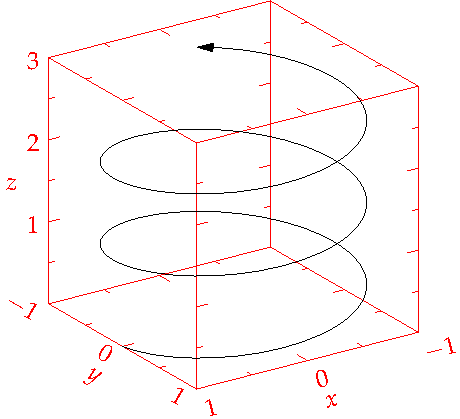
\includegraphics[width=\linewidth]{helix}
  \caption{This is a margin figure.  The helix is defined by
  $x = \cos(2\pi z)$, $y = \sin(2\pi z)$, and $z = [0, 2.7]$.  The figure was
  drawn using Asymptote (\url{http://asymptote.sf.net/}).}
  \label{fig:marginfig}
\end{marginfigure}
\begin{Verbatim}
  \begin{marginfigure}
    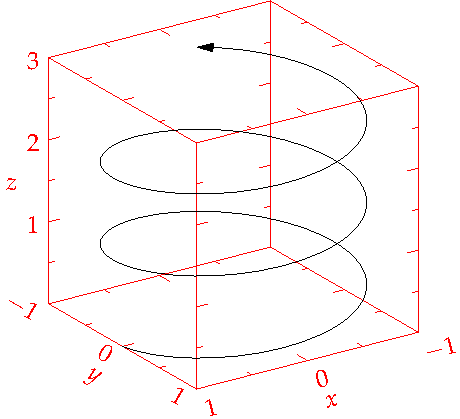
\includegraphics{helix}
    \caption{This is a margin figure.}
  \end{marginfigure}
\end{Verbatim}

The \docenv{marginfigure} and \docenv{margintable} environments accept an
optional parameter \docopt{offset} that adjusts the vertical position of the
figure or table. See the ``\nameref{sec:sidenotes}'' section above for
examples. The specifications are:
\begin{docspec}
  \doccmd{begin\{marginfigure\}[\docopt{offset}]}\\
  \qquad\ldots\\
  \doccmd{end\{marginfigure\}}\\
  \mbox{}\\
  \doccmd{begin\{margintable\}[\docopt{offset}]}\\
  \qquad\ldots\\
  \doccmd{end\{margintable\}}\\
\end{docspec}

Figure~\ref{fig:fullfig} is an example of the \Verb|figure*| environment and
figure~\ref{fig:textfig} is an example of the normal \Verb|figure| environment.

\begin{figure*}[h]
  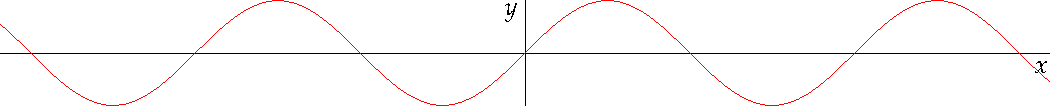
\includegraphics[width=\linewidth]{sine.pdf}%
  \caption{This graph shows $y = \sin x$ from about $x = [-10, 10]$.
  \emph{Notice that this figure takes up the full page width.}}%
  \label{fig:fullfig}%
\end{figure*}

\begin{figure}
  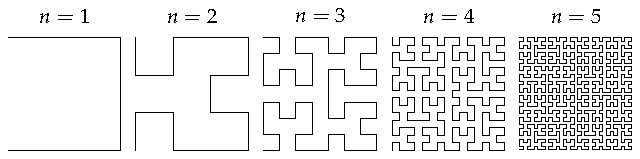
\includegraphics{hilbertcurves.pdf}
  %  \checkparity This is an \pageparity\ page.%
  \caption{Hilbert curves of various degrees $n$.
    \emph{Notice that this figure only takes up the main textblock width.}}
  \label{fig:textfig}
  %\zsavepos{pos:textfig}
  \setfloatalignment{b}
\end{figure}

Table~\ref{tab:normaltab} shows table created with the \docpkg{booktabs}
package. Notice the lack of vertical rules---they serve only to clutter the
table's data.

\begin{table}[ht]
  \centering
  \fontfamily{ppl}\selectfont
  \begin{tabular}{ll}
    \toprule
    Margin                    & Length                          \\
    \midrule
    Paper width               & \unit[8\nicefrac{1}{2}]{inches} \\
    Paper height              & \unit[11]{inches}               \\
    Textblock width           & \unit[6\nicefrac{1}{2}]{inches} \\
    Textblock/sidenote gutter & \unit[\nicefrac{3}{8}]{inches}  \\
    Sidenote width            & \unit[2]{inches}                \\
    \bottomrule
  \end{tabular}
  \caption{Here are the dimensions of the various margins used in the Tufte-handout class.}
  \label{tab:normaltab}
  %\zsavepos{pos:normaltab}
\end{table}
\subsection{References}
References are placed alongside their citations as sidenotes, as well. This can
be accomplished using the normal \Verb|\cite| command.\sidenote{The first
  paragraph of this document includes a citation.}

The complete list of references may also be printed automatically by using the
\Verb|\bibliography| command. (See the end of this document for an example.) If
you do not want to print a bibliography at the end of your document, use the
\Verb|\nobibliography| command in its place.

To enter multiple citations at one location,\cite{Tufte2006,Tufte1990} you can
provide a list of keys separated by commas and the same optional vertical
offset argument: \Verb|\cite{Tufte2006,Tufte1990}|.
\begin{docspec}
  \doccmd{cite[\docopt{offset}]\{\docarg{bibkey1,bibkey2,\ldots}\}}
\end{docspec}

\section{Full-width text blocks}

In addition to the new float types, there is a \docenv{fullwidth} environment
that stretches across the main text block and the sidenotes area.

\begin{Verbatim}
  \begin{fullwidth}
    Lorem ipsum dolor sit amet...
  \end{fullwidth}
\end{Verbatim}

\begin{fullwidth}
  \small\itshape\lipsum[1]
\end{fullwidth}

\section{Typography}\label{sec:typography}

\subsection{Typefaces}\label{sec:typefaces}
If the Palatino, \textsf{Helvetica}, and \texttt{Bera Mono} typefaces are
installed, this style will use them automatically. Otherwise, we'll fall back
on the Computer Modern typefaces.

\subsection{Letterspacing}\label{sec:letterspacing}
This document class includes two new commands and some improvements on existing
commands for letterspacing.

When setting strings of \allcaps{ALL CAPS} or \smallcaps{small caps}, the
letter\-spacing---that is, the spacing between the letters---should be
increased slightly.\cite{Bringhurst2005} The \Verb|\allcaps| command has proper
letterspacing for strings of \allcaps{FULL CAPITAL LETTERS}, and the
\Verb|\smallcaps| command has letterspacing for \smallcaps{small capital
  letters}. These commands will also automatically convert the case of the text
to upper- or lowercase, respectively.

The \Verb|\textsc| command has also been redefined to include letterspacing.
The case of the \Verb|\textsc| argument is left as is, however. This allows one
to use both uppercase and lowercase letters: \textsc{The Initial Letters Of The
  Words In This Sentence Are Capitalized.}

\section{Installation}\label{sec:installation}
To install the Tufte-\LaTeX\ classes, simply drop the following files into the
same directory as your \texttt{.tex} file:
\begin{quote}
  \ttfamily
  tufte-common.def\\
  tufte-handout.cls\\
  tufte-book.cls
\end{quote}

% TODO add instructions for installing it globally

\section{More Documentation}\label{sec:more-doc}
For more documentation on the Tufte-\LaTeX{} document classes (including
commands not mentioned in this handout), please see the sample book.

\section{Support}\label{sec:support}

The website for the Tufte-\LaTeX\ packages is located at
\url{http://code.google.com/p/tufte-latex/}. On our website, you'll find links
to our \smallcaps{svn} repository, mailing lists, bug tracker, and
documentation.

\bibliography{sample-handout}
\bibliographystyle{plainnat}

\end{document}